\documentclass[letterpaper,journal]{IEEEtran}
\usepackage{amsmath,amsfonts}
\usepackage{algorithmic}
\usepackage{algorithm}
\usepackage{array}
\usepackage[caption=false,font=normalsize,labelfont=sf,textfont=sf]{subfig}
\usepackage{textcomp}
\usepackage{stfloats}
\usepackage{url}
\usepackage{graphicx}
\usepackage{cite}
\usepackage{booktabs}
\usepackage{multirow}
\usepackage{xcolor}
\usepackage{amssymb}
\usepackage{pifont}
\usepackage{microtype}
\Urlmuskip=0mu plus 6mu\relax
\hyphenation{op-tical net-works semi-conduc-tor IEEE-Xplore}

\begin{document}

\title{GeoViewMiner-SAM2: Geometry-Guided Satellite--UAV Fusion with Explicit Prompt Mining for Building Instance Segmentation}

\author{Anonymous~Author,~\IEEEmembership{Member,~IEEE}
\thanks{Manuscript submitted to IEEE JSTAR, July 2026.}}

\markboth{IEEE Journal of Selected Topics in Applied Earth Observations and Remote Sensing}%
{Author \MakeLowercase{\textit{et al.}}: GeoViewMiner-SAM2: Geometry-Guided Satellite--UAV
Fusion}

\maketitle

\begin{abstract}
Building instance segmentation in overhead imagery remains challenging for small buildings,
weak roof boundaries, and adjacent instances. Prior satellite--street-view work shows that,
with geometric alignment, perspective observations can complement satellite representations for
cross-view semantic segmentation. UAV imagery can therefore serve as an auxiliary perspective
source for satellite-view building instances. However, existing satellite--UAV benchmarks focus
mainly on geo-localization and image retrieval, with supervision defined at the image or scene
level rather than for individual buildings. They therefore cannot evaluate whether UAV
observations with known camera parameters improve detection and mask delineation in an overhead
satellite view. We introduce \emph{SynSU-Build}, a controlled paired benchmark based on the UE5
City Sample. Its 1,500 aligned groups contain 9,000 RGB images: one synthetic satellite-like
image and five UAV images with renderer-provided intrinsics and poses per group, with
approximately 32.7k satellite-view building annotations in total. \emph{PromptMiner-SAM2} combines
a two-stage detector with explicit SAM2 prompts: it refines a supervised coarse mask with local
high-resolution features and converts it into foreground--background points and a dense mask
prompt, while the proposal supplies the box prompt. \emph{GeoViewMiner-SAM2} extends this
satellite-view pathway by using UAV intrinsics and poses to project a satellite-aligned ground-plane
grid into multiple UAV images, sampling local multi-scale UAV features around the projected
locations, and fusing the aggregated UAV features into the satellite-view feature pyramid through
zero-initialized residual paths. It requires UAV intrinsics, world-to-camera poses, and a
satellite-view pixel-to-ground mapping, but not a satellite-view pinhole model, explicit depth, or
building-height supervision. PromptMiner-SAM2 obtains a mask AP of 0.735 on WHU. On
SynSU-Build, GeoViewMiner-SAM2 obtains a mask AP of 0.721, 0.039 higher than that of an
independently trained single-stream reference. Together, SynSU-Build, PromptMiner-SAM2, and
GeoViewMiner-SAM2 define a paired benchmark and reference models for evaluating geometry-guided
fusion of UAV features for satellite-view building instance segmentation.
\end{abstract}

\begingroup
\hbadness=10000
\begin{IEEEkeywords}
Building instance segmentation, SAM2, PromptMiner-SAM2, GeoViewMiner-SAM2, satellite--UAV
fusion, cross-view learning.
\end{IEEEkeywords}
\endgroup


%==============================================================================
\section{Introduction}
%==============================================================================
\IEEEPARstart{R}{emote} sensing instance segmentation detects and delineates individual objects
in overhead imagery for cadastral mapping, urban planning, disaster response, and map updating.
For buildings, the task requires more than separating built-up land from its surroundings:
adjacent structures must be distinguished and their individual boundaries recovered. This is
difficult when roofs are small, weakly contrasted, shadowed, or separated by narrow gaps. Even
when an overhead image supplies broad spatial coverage, it may not contain sufficient visual
detail to resolve these ambiguities, which motivates the use of complementary perspective
observations.

Prior work on satellite--street-view fusion shows that geometrically aligned street-view
observations can complement satellite representations for map-view semantic
segmentation~\cite{ref_sgbeyv,ref_crffnet}. UAV imagery provides nearby oblique observations of the same
scene for an overhead building task. However, complementary imagery cannot simply be
concatenated with the satellite-view representation. The two views differ in scale, viewing
direction, and perspective; their correspondence also varies across the scene. A useful
cross-view model must therefore identify where UAV features belong in the overhead satellite
view while preserving the latter as the domain in which boxes and instance masks are predicted.

Existing satellite--UAV benchmarks already provide paired observations, but they are designed
mainly for retrieval and geo-localization, with supervision defined by image identity, scene
association, or geographic position~\cite{ref_university,ref_denseuav,ref_unigeo}. Such supervision can
establish where an image was captured, but not which UAV observations support the boundary of a
particular overhead-view building. Conversely, satellite--street-view semantic segmentation
studies demonstrate dense geometric fusion~\cite{ref_sgbeyv,ref_crffnet}, yet semantic maps do not require
the separation of neighboring instances. These settings therefore leave open a more specific question: when
per-view camera parameters are known, can UAV observations improve the detection and
delineation of individual buildings in an overhead satellite view?

We examine this question through \emph{SynSU-Build}, a controlled benchmark comprising 1,500
aligned synthetic scene groups. Each group contains one satellite-like nadir image, five
oblique UAV images with renderer-provided intrinsics and poses, and building-instance
supervision for the satellite view. Synthetic construction makes the scene pairing, camera
geometry, and satellite-view annotations jointly available, while avoiding confounding changes
in sensors, acquisition time, metadata, and camera recovery that arise in real collections.

This setting requires both a capable satellite-view segmenter and a geometry-aware mechanism
for incorporating UAV features. We build the shared satellite-view pathway on
SAM2~\cite{ref_sam2}, which retains SAM's promptable segmentation interface~\cite{ref_sam} and
provides a hierarchical image encoder with multi-resolution features that can be shared by the
two-stage detection pathway and prompt-conditioned mask decoding. \emph{PromptMiner-SAM2}
establishes this pathway: it predicts a proposal-conditioned coarse shape, converts that shape
into explicit point, box, and dense-mask prompts for SAM2, and uses local high-resolution
features to refine uncertain boundaries. \emph{GeoViewMiner-SAM2} extends this pathway by using
UAV intrinsics and poses to project a satellite-aligned ground-plane grid into multiple UAV
images, sampling local multi-scale UAV features around the projected locations, and fusing the
aggregated UAV features into the satellite-view feature pyramid through zero-initialized
residual paths. The shared satellite-view pathway isolates the complete geometry-guided
cross-view extension from unrelated architectural changes.

\subsection{Contributions}

We make three contributions:
\begin{enumerate}
\item \textbf{SynSU-Build, a synthetic satellite--UAV building instance segmentation
      benchmark,} whose 1,500 aligned groups provide a synthetic satellite-like image, five UAV
      images with renderer-provided intrinsics and poses, and satellite-view building-instance
      masks for each scene.

\item \textbf{PromptMiner-SAM2, a boundary-aware explicit-prompt architecture,} which converts
      a supervised proposal-conditioned coarse shape into native point, box, and dense-mask
      prompts and applies constrained local high-resolution refinement before prompt encoding,
      thereby defining the satellite-view pathway for the paired setting.

\item \textbf{GeoViewMiner-SAM2, a geometry-guided dual-stream model,} which projects a
      satellite-aligned ground-plane grid into UAV images using their known camera parameters,
      aggregates local multi-scale UAV features, and fuses them into the satellite-view feature
      pyramid through zero-initialized residual paths.
\end{enumerate}

The remainder of this paper is organized as follows. Section~\ref{sec:related} reviews related
work; Section~\ref{sec:dataset} introduces SynSU-Build; Section~\ref{sec:method} presents the
single-stream satellite-view model and its dual-stream extension; Section~\ref{sec:experiments}
reports the experimental setup and results; Section~\ref{sec:discussion} discusses the
findings; and Section~\ref{sec:conclusion} concludes the paper.

%==============================================================================
\section{Related Work}
\label{sec:related}
%==============================================================================

\subsection{Synthetic Data for Remote Sensing}
Synthetic rendering is useful when aerial acquisition, controlled multi-view capture, or dense
annotation is costly. Synthinel-1~\cite{ref_synthinel} provides synthetic overhead imagery and
building labels for building segmentation and synthetic-to-real transfer.
UrbanScene3D~\cite{ref_urbanscene3d} combines reconstructed urban regions with Unreal Engine
and AirSim environments, providing varied observation patterns, depth, LiDAR, bounding boxes,
and building identities. SkyScenes~\cite{ref_skyscenes} broadens the range of synthetic UAV
scenes and dense labels, while UEMM-Air~\cite{ref_uemmair} provides aligned multimodal UAV
observations for multiple perception tasks. At the satellite scale, SynRS3D~\cite{ref_synrs3d}
supports land-cover mapping, height estimation, and building change detection, and
GTA-UAV~\cite{ref_gtauav} shows that game environments can produce large continuous regions for
UAV geo-localization.

These datasets show the value of controllable rendering and automatic labels, but they are not
designed to jointly provide paired satellite--UAV observations, satellite-view building-instance
supervision, and usable per-view camera parameters. Table~\ref{tab:dataset_comparison} compares
the three properties required here: paired satellite--UAV observations, satellite-view instance
supervision, and per-view camera parameters. Together, they allow features from auxiliary UAV
views to be related to individual buildings in an overhead satellite view.

\subsection{Remote Sensing Instance Segmentation}
Remote sensing instance segmentation builds on both general-purpose and remote-sensing-specific
designs. Mask R-CNN~\cite{ref_maskrcnn} adds a parallel mask branch to Faster R-CNN, and
Cascade R-CNN~\cite{ref_cascade} improves proposal quality through cascaded stages with
increasing IoU thresholds. HTC~\cite{ref_htc} further interleaves detection and segmentation
stages, whereas HQ-ISNet~\cite{ref_hqisnet} emphasizes high-resolution and multi-level feature
propagation for small, densely distributed targets. Boundary-oriented methods address a
complementary difficulty: PointRend~\cite{ref_pointrend} predicts adaptively sampled uncertain
points, while P2PFormer~\cite{ref_p2pformer} segments geometric primitives and predicts their
order to form building polygons. Mask2Former~\cite{ref_mask2former} instead uses a set of mask
queries and masked attention for universal segmentation.

Promptable foundation models introduce a category-agnostic mask prior, but dense instance
prediction requires an automatic prompting mechanism. For remote sensing, zero- and one-shot
experiments report that SAM performance depends on image scale and prompt
design~\cite{ref_samrsapp}; SAMRS~\cite{ref_samrs} combines SAM with existing remote-sensing
object-detection datasets to construct large-scale segmentation data.
RSPrompter~\cite{ref_rsprompter} maps instance features to learned prompt embeddings, MC-SAM
SEG~\cite{ref_mcsamseg} adapts the encoder with task-specific visual modules, and
RS4D~\cite{ref_rs4d} distills knowledge from a visual foundation model into a linear-time
state-space backbone for efficient instance segmentation. PromptMiner-SAM2 instead retains the
native geometric prompt interface and constructs point, box, and dense-mask prompts from a
supervised proposal-conditioned shape.

Coarse-mask refinement provides a related route to improving mask quality.
CascadePSP~\cite{ref_cascadepsp} combines global and local refinement,
SegRefiner~\cite{ref_segrefiner} formulates refinement as a discrete denoising process, and
SAMRefiner~\cite{ref_samrefiner} derives prompts from an input coarse mask. In contrast, our
coarse shape is an internal instance-conditioned representation learned jointly with detection;
P2BoundaryRefiner is limited to a predicted boundary neighborhood before this shape is
converted into SAM2 prompts.

\subsection{Cross-View Learning}
Satellite--UAV cross-view learning has mainly been studied through retrieval and
geo-localization. University-1652~\cite{ref_university} provides matched satellite, synthetic
UAV, and ground observations for drone-view target localization and navigation, and
DenseUAV~\cite{ref_denseuav} moves to real low-altitude urban UAV imagery with dense spatial
sampling and joint retrieval/localization evaluation. More generally,
TransGeo~\cite{ref_transgeo} shows that transformer-based global correlation can support
cross-view geo-localization without hand-crafted polar alignment. The satellite--UAV benchmarks
provide image-level matching or position supervision, rather than correspondences between UAV
observations and individual overhead-view building instances.

A second line of work uses known camera geometry to transform perspective observations into a
canonical top-down representation. Cross-View Transformers~\cite{ref_cvt} use camera intrinsics
and extrinsics in map-view semantic segmentation from multi-camera images. In remote sensing,
SG-BEV~\cite{ref_sgbeyv} projects street-view features into BEV space and fuses them with
satellite features for fine-grained building-attribute semantic segmentation. These studies
motivate geometry-guided feature transfer, but their outputs are semantic maps and their paired
observations are satellite--street-view rather than satellite--UAV.

Neither direction establishes a satellite--UAV pathway for overhead building instance
segmentation. GeoViewMiner-SAM2 therefore retains the satellite-view instance pathway described
above and uses renderer-provided UAV intrinsics and poses to localize UAV features before
feature fusion. In this way, the dual-stream model extends the single-stream segmentation path
rather than replacing it with an image-level matching objective.

\section{Dataset}
\label{sec:dataset}
%==============================================================================

SynSU-Build comprises 1,500 aligned scene groups. Each group contains one synthetic
satellite-like image with building-instance masks and five oblique UAV RGB images with
renderer-provided intrinsics and world-to-camera poses. Table~\ref{tab:dataset_comparison}
compares this setting with established single-view instance-level benchmarks and representative
cross-view or synthetic remote sensing datasets. The former provide established overhead
instance labels, whereas the latter provide multiple views, controllable rendering, or camera
information but generally lack satellite-view instance supervision.

\begin{table*}[!t]
\caption{Comparison with Representative Instance-Level, Cross-View, and Synthetic Remote Sensing Datasets}
\label{tab:dataset_comparison}
\centering
\scriptsize
\setlength{\tabcolsep}{3.2pt}
\renewcommand{\arraystretch}{1.12}
\begin{tabular*}{\textwidth}{@{\extracolsep{\fill}}lcccccccl@{}}
\toprule
Dataset & Source & Views & S--U Pair & Multi-UAV & Camera $K/T$ & Aux./3D Inst. & Eval. Inst. & Primary Task \\
\midrule
\multicolumn{9}{l}{\textit{Single-view instance and building-footprint datasets}} \\
iSAID~\cite{ref_isaid} & Real & A & \ding{55} & \ding{55} & \ding{55} & \ding{55} & \ding{51} & Instance segmentation \\
WHU Building~\cite{ref_whu} & Real & A/S & \ding{55} & \ding{55} & \ding{55} & \ding{55} & \ding{51} & Instance segmentation \\
SpaceNet Buildings~\cite{ref_spacenet} & Real & S & \ding{55} & \ding{55} & \ding{55} & \ding{55} & \ding{51} & Building footprints \\
xBD~\cite{ref_xbd} & Real & S/T & \ding{55} & \ding{55} & $\triangle$ & \ding{55} & \ding{51} & Damage assessment \\
\midrule
\multicolumn{9}{l}{\textit{Cross-view and synthetic remote sensing datasets}} \\
University-1652~\cite{ref_university} & Hybrid & S/U/G & \ding{51} & \ding{51} & \ding{55} & \ding{55} & \ding{55} & Geo-localization \\
DenseUAV~\cite{ref_denseuav} & Real & S/U & \ding{51} & \ding{51} & $\triangle$ & \ding{55} & \ding{55} & Geo-localization \\
GTA-UAV~\cite{ref_gtauav} & Synthetic & S/U & $\triangle$ & $\triangle$ & $\triangle$ & \ding{55} & \ding{55} & Geo-localization \\
UrbanScene3D~\cite{ref_urbanscene3d} & Hybrid & U/3D & \ding{55} & $\triangle$ & $\triangle$ & \ding{51} & \ding{55} & Reconstruction/3D inst. \\
SkyScenes~\cite{ref_skyscenes} & Synthetic & U & \ding{55} & \ding{55} & $\triangle$ & \ding{51} & \ding{51} & Scene understanding \\
UEMM-Air~\cite{ref_uemmair} & Synthetic & U/MM & \ding{55} & \ding{55} & $\triangle$ & \ding{51} & \ding{51} & Multimodal perception \\
SynRS3D~\cite{ref_synrs3d} & Synthetic & S & \ding{55} & \ding{55} & \ding{55} & \ding{55} & \ding{55} & Semantic/height \\
\midrule
\textbf{SynSU-Build} & Synthetic & S/U & \ding{51} & \ding{51} & \ding{51} & \ding{55} & \ding{51} & Instance segmentation \\
\bottomrule
\multicolumn{9}{l}{\footnotesize A: aerial; S: satellite; U: UAV; G: ground; T: temporal; MM: multimodal; S--U Pair: scene-level association.} \\
\multicolumn{9}{l}{\footnotesize Multi-UAV: multiple UAV observations per associated scene; $K/T$: per-view intrinsics and metric extrinsics.} \\
\multicolumn{9}{l}{\footnotesize Eval. Inst.: masks or polygons in the evaluated overhead or aerial image.} \\
\multicolumn{9}{l}{\footnotesize \ding{51}: available; \ding{55}: unavailable; $\triangle$: incomplete pairing or metadata without full per-view $K/T$.}
\end{tabular*}
\end{table*}

\noindent\textit{Scene and spatial sampling.}
We build SynSU-Build on the UE5 City Sample, whose contiguous urban coverage, stable building
actors, programmable cameras, and deterministic rendering support paired satellite--UAV
acquisition~\cite{ref_citysample}. UE5 World Partition provides streamable spatial cells while
preserving a shared world coordinate system~\cite{ref_worldpartition}. We sample candidate
centers on a coarse spatial grid and reject locations with insufficient nearby urban structure
using actor-based content filtering. Table~\ref{tab:synsu_configuration} lists the sampling,
camera, and dataset-scale settings.

Figure~\ref{fig:sampling_pipeline} illustrates the spatial sampling strategy, the
satellite--UAV camera arrangement, and the synthetic satellite-view instance annotations generated
for each accepted center.

\begin{figure}[!t]
\centering
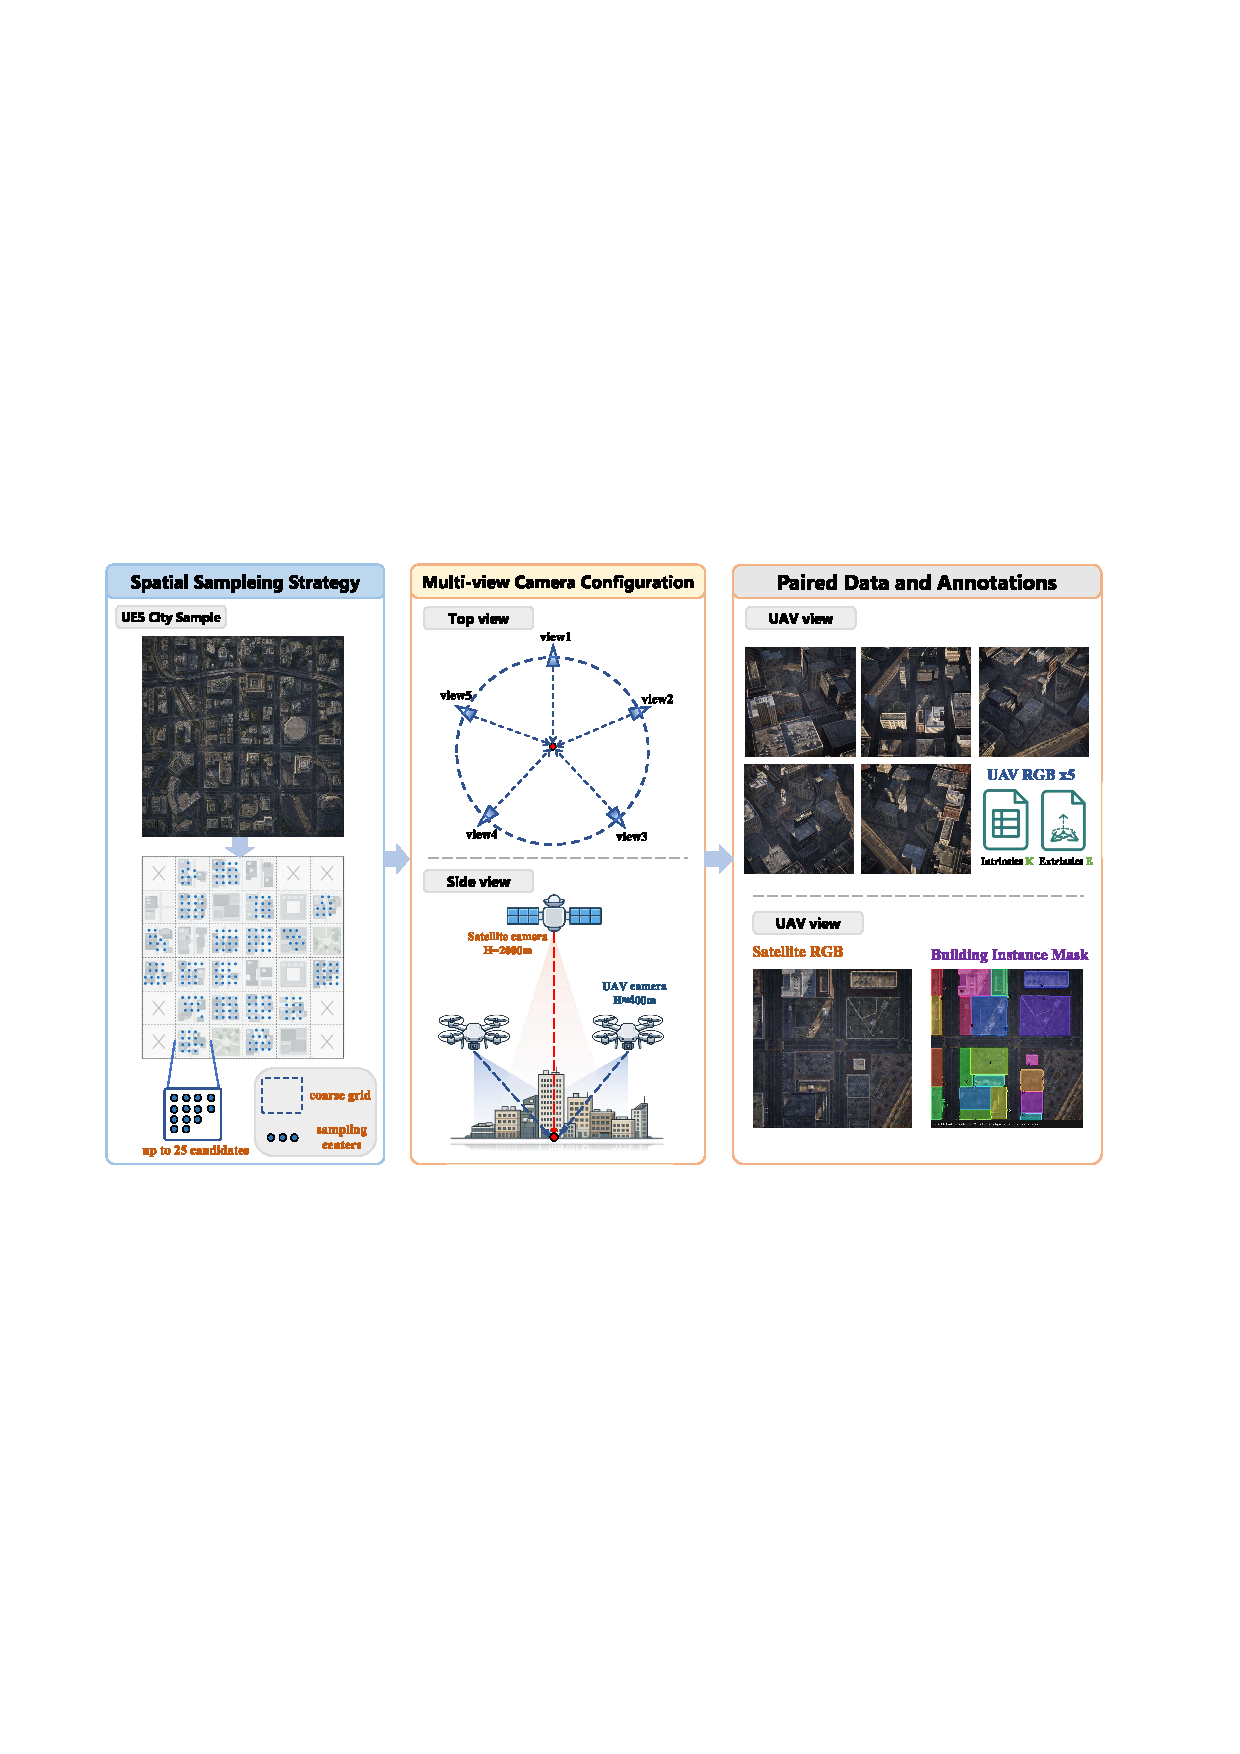
\includegraphics[width=\columnwidth]{采样示例图.pdf}
\caption{Overview of the SynSU-Build sampling and rendering pipeline. Left: urban sampling uses a coarse spatial grid with up to 25 candidate centers per cell and content-based filtering. Middle: five oblique UAV cameras surround a common scene center, while one synthetic satellite-like camera observes it from nadir. Right: each accepted group contains five unannotated UAV RGB images with camera parameters and a paired satellite-like RGB image with its building instance mask.}
\label{fig:sampling_pipeline}
\end{figure}

\noindent\textit{Camera configuration.}
Each accepted center is observed by one nadir satellite-view camera and five evenly distributed
oblique UAV cameras directed toward the same urban region. The UAV views share one intrinsic
configuration, and their renderer-provided world-to-camera poses provide complementary azimuths
around the scene centre. The nadir pinhole rendering approximates satellite-scale ground coverage but
does not reproduce the full imaging physics of an orbital sensor; we therefore refer to it as a
\emph{synthetic satellite-like view}. All six cameras are expressed in the same metric frame,
enabling geometric transformation of UAV observations to the satellite-image/world reference.

\noindent\textit{Instance annotation.}
City Sample buildings can comprise multiple mesh actors. Mesh components assigned to the same
rendered building are combined under one frame-local instance label. The satellite-view annotation is
the visible building region in the satellite-like nadir view; its instance-ID layer shares the
same camera frame as the RGB image and is converted into binary masks, bounding boxes, areas,
and COCO-format records. The UAV views provide RGB imagery and renderer-provided camera
parameters only, without pixel-level labels or cross-view instance IDs.

\noindent\textit{Dataset scale.}
The finalized benchmark contains 1,500 aligned groups and approximately 32.7k satellite-view
building-instance occurrences. Counts refer to image-level annotations rather than spatially
deduplicated physical buildings, and all partitions are defined at group level to keep the six
associated views together.

\begin{table}[!t]
\caption{SynSU-Build Sampling and Camera Configuration}
\label{tab:synsu_configuration}
\centering
\footnotesize
\setlength{\tabcolsep}{4pt}
\renewcommand{\arraystretch}{1.06}
\begin{tabular}{p{0.38\columnwidth}p{0.54\columnwidth}}
\toprule
Configuration item & Setting \\
\midrule
Spatial candidate policy & Coarse grid; up to 25 candidates per cell; actor-based filtering \\
Accepted scene groups & 1,500 \\
Views per group & 1 nadir satellite + 5 oblique UAV \\
Native image resolution & $512\times512$ pixels for all views \\
UAV azimuths & $0^{\circ}$, $72^{\circ}$, $144^{\circ}$, $216^{\circ}$, $288^{\circ}$ \\
UAV orbit / altitude / pitch & 300~m / 400~m / perturbation within $\pm5^{\circ}$ \\
UAV optics & 55.4-mm focal length; 36-mm square sensor \\
Satellite-view camera & Nadir; 2,000-m altitude; 200-mm focal length; 36-mm square sensor \\
Satellite coverage / nominal GSD & Approx. $360\times360$~m / 0.70~m per pixel \\
Exported UAV geometry & Intrinsics $K_v$ and world-to-camera pose $T_v^{w\rightarrow c}$ (UE centimetres) \\
Dataset scale & 9,000 RGB images; approx. 32.7k satellite-view instances; 21.8 instances per annotated satellite image \\
Train/validation/test split & 1,200 / 150 / 150 groups (8:1:1) \\
\bottomrule
\end{tabular}
\end{table}

%==============================================================================
\section{Method}
\label{sec:method}
%==============================================================================

PromptMiner-SAM2 and GeoViewMiner-SAM2 share the satellite-view instance-segmentation pathway
defined for SynSU-Build. Given a satellite-view image, PromptMiner-SAM2 predicts candidate boxes
and masks from that view alone. GeoViewMiner-SAM2 additionally receives UAV RGB images with
renderer-provided intrinsics and world-to-camera poses, which it uses with a satellite-view
pixel-to-ground mapping to sample auxiliary UAV features in the feature pyramid. Both models
produce boxes and masks in the satellite view.

\subsection{PromptMiner-SAM2: Explicit Prompt Mining from Coarse Shapes}
\label{sec:single_method}

PromptMiner-SAM2 adapts the interactive SAM2 image-segmentation pipeline for automatic instance
segmentation. Its detection path first identifies candidate instances and supplies proposal
boxes. For each candidate, a coarse-mask branch predicts a proposal-conditioned shape, and a
boundary-refinement step uses high-resolution $P_2$ features near the predicted contour. The
refined shape provides foreground--background points and a dense-mask prompt, while the proposal
box provides the box prompt. The pretrained PromptEncoder and SAM2 MaskDecoder process these
native prompts to produce the final instance mask.

\subsubsection{Overall Architecture}
For a $1024\times1024$ image, the SAM2 Hiera-Base+ encoder produces hierarchical features at
strides $\{4,8,16,32\}$. A detection-oriented PAFPN converts them into pyramid levels
$\{P_2,\ldots,P_6\}$ for proposal generation and box prediction. The SAM2 image embedding and
higher-resolution decoder features are retained for prompt-conditioned mask decoding. The
pretrained image encoder therefore serves both instance discovery and SAM2-based mask
prediction.

\begin{figure*}[!t]
\centering
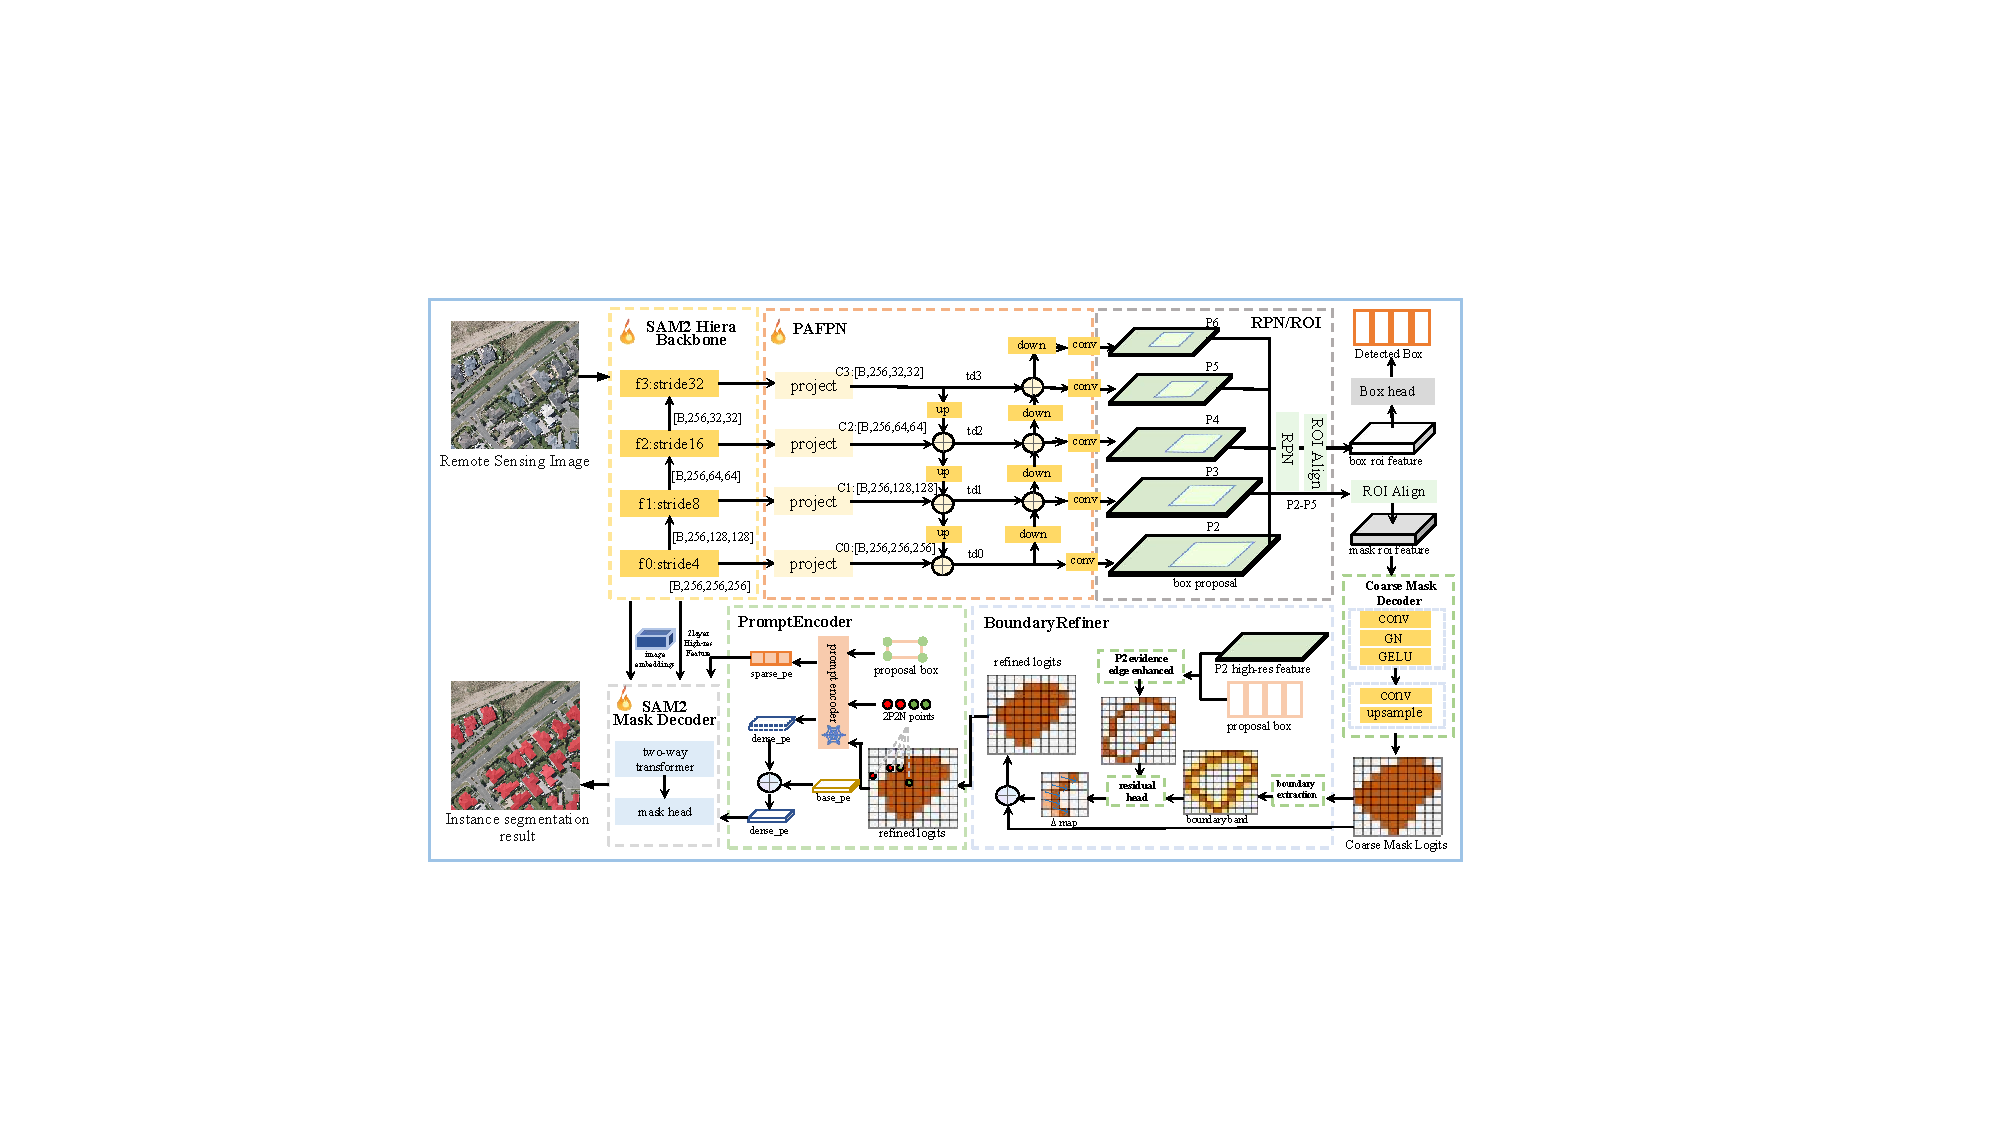
\includegraphics[width=\textwidth]{单流模型.pdf}
\caption{Architecture of PromptMiner-SAM2. The SAM2 Hiera backbone feeds a PAFPN, RPN, and RoI heads for proposal discovery. For each mask RoI, the coarse-mask decoder predicts proposal-conditioned shape logits. P2BoundaryRefiner uses high-resolution $P_2$ features only in a predicted boundary neighborhood to produce refined logits. The resulting foreground--background points, proposal box, and dense mask are encoded as native SAM2 prompts; together with the SAM2 image embedding and high-resolution features, they are decoded into the final instance mask.}
\label{fig:single_architecture}
\end{figure*}

Figure~\ref{fig:single_architecture} shows this procedure. The upper path supplies multi-scale
detection features and candidate boxes; the lower path converts each proposal-conditioned shape
into explicit sparse and dense prompts. The shared image encoder and proposal geometry link the
two paths while retaining SAM2's native prompt interface.

Let $b_r$ denote the candidate box used by the mask branch: a sampled positive proposal during
training and a final detected box during inference. Multi-level RoIAlign extracts a
$14\times14$ mask feature $X_r\in\mathbb{R}^{512\times14\times14}$ from $P_2$--$P_5$. The same
$b_r$ defines the coordinate frame for mask feature extraction, coarse-mask supervision,
point-coordinate conversion, dense-mask placement, and the SAM2 box prompt. This shared
geometry keeps all prompt modalities aligned with the instance being decoded.

\subsubsection{Proposal-Conditioned Coarse Shape}
The Explicit Coarse-Prompt Miner begins by representing each candidate instance with an
explicitly supervised intermediate mask rather than mapping $X_r$ directly to unconstrained
prompt embeddings. A lightweight convolutional decoder with two upsampling stages predicts
\begin{equation}
C_r=f_{\mathrm{coarse}}(X_r), \qquad
C_r\in\mathbb{R}^{1\times64\times64}.
\label{eq:coarse_logits}
\end{equation}
Let $G_r\in\{0,1\}^{H_c\times W_c}$ denote the corresponding ground-truth instance cropped by
$b_r$ and resized with nearest-neighbor interpolation, where $H_c=W_c=64$. Binary cross-entropy
and Dice losses directly supervise $C_r$, making the intermediate geometry inspectable and
separately supervised from the final decoder output.

\subsubsection{P2 Boundary Refinement}
The coarse decoder infers an entire instance from a fixed $14\times14$ RoI feature.
P2BoundaryRefiner introduces higher-resolution $P_2$ features, but restricts its correction to
a support derived from the coarse prediction rather than learning a second global mask. Let
$\operatorname{sg}(\cdot)$ denote stop-gradient. It first obtains an uncertainty map and a
one-pixel boundary from the raw coarse prediction:
\begin{equation}
\begin{aligned}
p_r&=\sigma(\operatorname{sg}(C_r)),\\
u_r&=4p_r(1-p_r),\\
K_r&=\partial\mathbf{1}[\operatorname{Avg}^{\mathrm{rep}}_3(p_r)\geq0.5],
\end{aligned}
\label{eq:p2_support}
\end{equation}
where $\operatorname{Avg}^{\mathrm{rep}}_3$ is replicate-padded $3\times3$ averaging,
$\partial$ extracts a one-pixel morphological boundary, and $\operatorname{Dilate}_k$ denotes
$k$ repeated dilations. The raw boundary band and residual search support are
\begin{equation}
R_r=\operatorname{Dilate}_2(K_r),\qquad
S_r=v_r\operatorname{Dilate}_4(K_r),
\label{eq:p2_bands}
\end{equation}
where $v_r=1$ only when the radius-four band is nonempty and covers at most half of the coarse
canvas; otherwise $v_r=0$. Thus, the forward support is computed from the prediction and
restricted to a local region.

A projection block reduces $P_2$ to a local $32\times32$ RoI feature at $b_r$. With
\begin{equation}
\begin{aligned}
Z_r&=\operatorname{RoIAlign}
\!\left(\Pi_2(\operatorname{sg}(P_2)),b_r\right),\\
H_r&=Z_r-\operatorname{Avg}^{\mathrm{rep}}_3(Z_r),
\end{aligned}
\end{equation}
the coarse-grid signals are first matched to the crop resolution:
\begin{equation}
\begin{aligned}
\bar p_r&=\mathcal{R}_{32}(p_r),\qquad
\bar u_r=\mathcal{R}_{32}(u_r),\\
\bar S_r&=\mathcal{A}_{32}(S_r),\\
V_r&=h_{\mathrm{fuse}}([Z_r,H_r,\bar p_r,\bar u_r,\bar S_r]),
\end{aligned}
\label{eq:p2_fusion}
\end{equation}
where $\mathcal{R}_{32}$ is bilinear resizing and $\mathcal{A}_{32}$ is adaptive max pooling.
The fused local representation is resized to $64\times64$ before the residual head predicts
\begin{equation}
\begin{aligned}
\Delta_r&=0.20\left\{2\tanh\!\left[
h_{\mathrm{res}}(\mathcal{U}_{64}(V_r))\right]\right\}\odot S_r,\\
\widehat C_r&=C_r+\Delta_r.
\end{aligned}
\label{eq:p2_refinement}
\end{equation}
Here $\mathcal{U}_{64}$ denotes bilinear upsampling. The residual $\Delta_r\in[-0.4,0.4]$ is
zero outside $S_r$. Because the residual head is zero initialized, the module initially leaves
the coarse prediction unchanged. For training, let $T_r=\operatorname{Dilate}_2(\partial G_r)$
and define
\begin{equation}
W_r=S_r\odot\max(R_r,T_r).
\label{eq:p2_loss_support}
\end{equation}
Here and below, products and maxima between masks are evaluated elementwise.
For valid instances $\mathcal{V}=\{r:\sum_{ij}W_{r,ij}>0\}$, the unweighted local objective is
\begin{equation}
\mathcal{L}_{\mathrm{p2}}=
\frac{1}{|\mathcal{V}|}\sum_{r\in\mathcal{V}}
\frac{\sum_{ij}W_{r,ij}\,\ell_{\mathrm{BCE}}
(\operatorname{sg}(C_{r,ij})+\Delta_{r,ij},G_{r,ij})}
{\sum_{ij}W_{r,ij}}.
\label{eq:p2_loss}
\end{equation}
with $\mathcal{L}_{\mathrm{p2}}=0$ when $\mathcal{V}$ is empty.
The target boundary affects the training loss support only; it never enters the forward support
$S_r$. When P2BoundaryRefiner is disabled, $\widehat C_r=C_r$, and the non-P2 variants
construct prompts directly from the raw coarse prediction.

\subsubsection{Explicit Prompt Mining and Decoding}
The Explicit Coarse-Prompt Miner converts $\widehat C_r$ into complementary sparse and dense
prompts. For sparse prompting, let $\widehat p_r=\sigma(\operatorname{sg}(\widehat C_r))$ and
define
\begin{equation}
d_r=\frac{\mathcal{D}_{\mathrm{morph}}(\mathbf{1}[\widehat p_r\geq0.5])}{\min(H_c,W_c)},
\qquad s_r^{+}=\widehat p_r\odot d_r,
\label{eq:point_mining_score}
\end{equation}
where $\mathcal{D}_{\mathrm{morph}}$ is the discrete interior distance obtained by iterative
morphological erosion. The adaptive 2P2N miner selects up to two foreground points from
confident interiors and up to two background points from the exterior of the predicted shape.
Confidence, topology, and spatial-separation rules keep points away from uncertain boundaries.
If a reliable point is unavailable, its slot is neutralized and the remaining prompts are used.
Valid local coordinates are mapped to image coordinates through $b_r$, which also supplies
SAM2's native two-corner box prompt.

For dense prompting, the refined coarse logits are used directly as a fixed dense prompt,
resized to the box extent, and rasterized on the native mask-input canvas of the PromptEncoder,
\begin{equation}
Q_r=\operatorname{Place}(\widehat C_r,b_r),
\label{eq:dense_canvas}
\end{equation}
where $\operatorname{Place}$ resizes the coarse logits to the candidate box on the native
mask-input canvas and fills the exterior with zero logits. Let $E_r^{\mathrm{mask}}$ be the
mask embedding produced by the frozen PromptEncoder, $E^0$ its frozen pretrained no-mask
embedding replicated over the dense grid, and $M_r$ the box support at the dense-embedding
resolution. The dense embedding supplied to the MaskDecoder is
\begin{equation}
D_r=E^0+\alpha M_r\odot
\left(E_r^{\mathrm{mask}}-E^0\right),
\qquad \alpha=\sigma(a),
\label{eq:dense_prompt_gate}
\end{equation}
where the learnable global gate is initialized with $\alpha=0.25$. The support mask confines
the dense correction to the candidate box. Points, the box, and $Q_r$ are passed together
through one frozen PromptEncoder call, retaining their native SAM2 semantics and jointly
encoding interior, exclusion, extent, and shape information.

For each candidate instance, the frozen PromptEncoder jointly encodes the point slots, box
corners, and $Q_r$; invalid point embeddings are zeroed. The image embedding is reused for all
instances in an image, and the higher-resolution SAM2 features follow the same instance order.
The trainable SAM2 MaskDecoder predicts logits $Y_r$, which are supervised on the crop defined
by $b_r$ during training and pasted using the final detected box at inference.

\subsubsection{Training Objective}

Let $\mathcal{I}$ be the sampled positive instances. The unweighted coarse objective is
\begin{equation}
\begin{aligned}
\mathcal{L}_{\mathrm{coarse}}
=\frac{1}{|\mathcal{I}|}\sum_{r\in\mathcal{I}}\Bigg[
&\frac{1}{H_cW_c}\sum_{ij}\ell_{\mathrm{BCE}}(C_{r,ij},G_{r,ij})\\
&+1-\frac{2\sum_{ij}\sigma(C_{r,ij})G_{r,ij}+\epsilon}
{\sum_{ij}\sigma(C_{r,ij})+\sum_{ij}G_{r,ij}+\epsilon}\Bigg],
\end{aligned}
\label{eq:coarse_loss}
\end{equation}
where $\epsilon=10^{-6}$ and the loss is zero when $\mathcal{I}$ is empty. The complete
single-stream objective is
\begin{equation}
\mathcal{L}=\mathcal{L}_{\mathrm{det}}
+\mathcal{L}_{\mathrm{mask}}
+0.10\mathcal{L}_{\mathrm{coarse}}
+0.05\mathcal{L}_{\mathrm{p2}}.
\label{eq:single_loss}
\end{equation}
Here $\mathcal{L}_{\mathrm{det}}$ contains the RPN classification and regression losses and the
RoI classification and box-regression losses. $\mathcal{L}_{\mathrm{mask}}$ is the standard
per-pixel binary mask loss on $Y_r$. The terms $\mathcal{L}_{\mathrm{coarse}}$ and
$\mathcal{L}_{\mathrm{p2}}$ denote the unweighted normalized objectives in
Eqs.~\eqref{eq:coarse_loss} and~\eqref{eq:p2_loss}; their weights are 0.10 and 0.05,
respectively. Ground truth enters P2BoundaryRefiner only through $\mathcal{L}_{\mathrm{p2}}$,
while the refinement support used in both training and inference is derived solely from the raw
prediction.

%==============================================================================
\subsection{GeoViewMiner-SAM2}
\label{sec:dual_method}
%==============================================================================

GeoViewMiner-SAM2 retains the PromptMiner-SAM2 satellite-view network and augments its feature
pyramid with UAV features aligned by the available camera parameters. The trainable satellite-view
encoder produces $\{P_2,\ldots,P_6\}$, while an independent frozen Hiera-Base+ encoder
processes the five UAV images. Their multi-scale features are sampled on a satellite-aligned
ground grid and aggregated with satellite $P_3$ queries. The resulting feature enters $P_2$ and
$P_3$ through zero-initialized residual paths, so the satellite-view model is recovered exactly at
initialization.

\begin{figure}[!t]
\centering
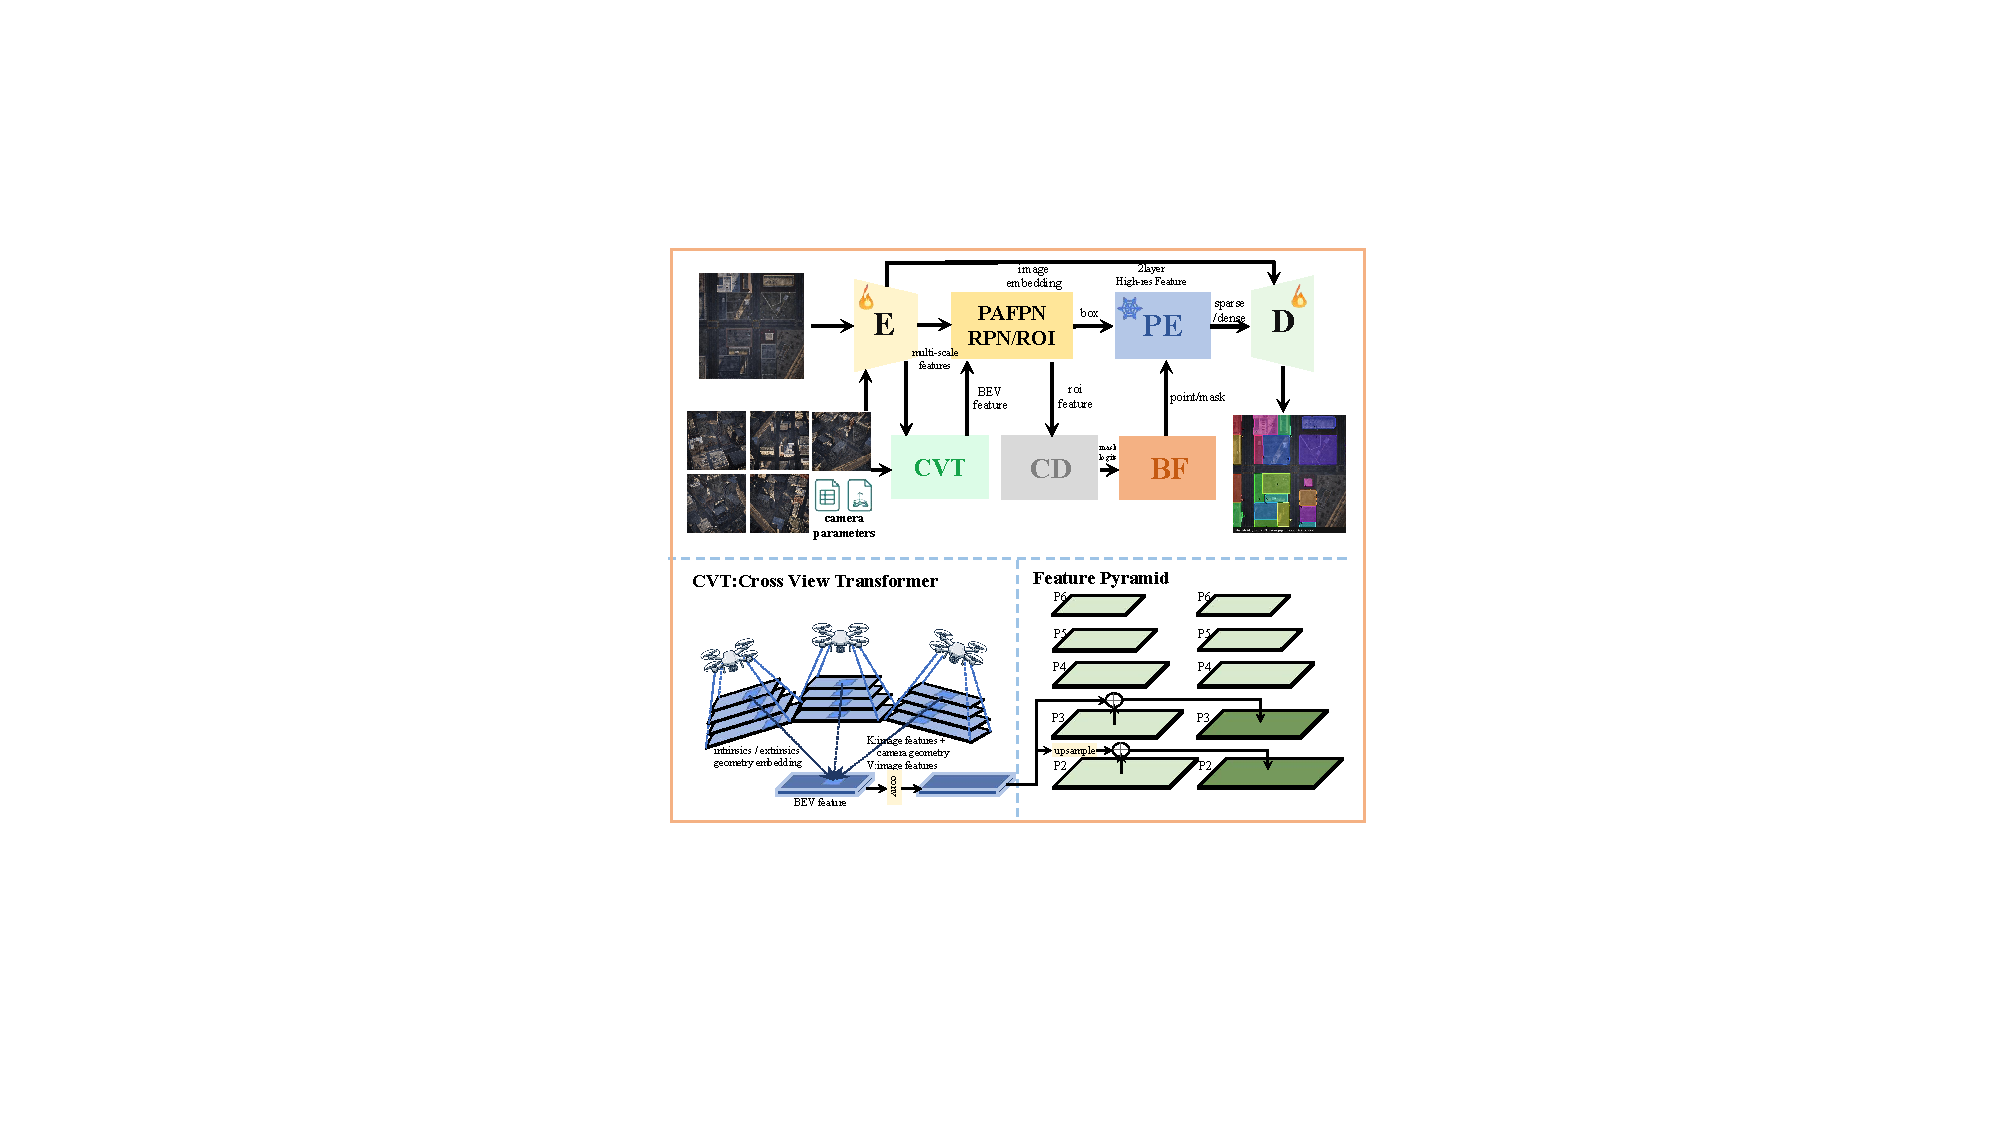
\includegraphics[width=\columnwidth]{双流模型.pdf}
\caption{Architecture of GeoViewMiner-SAM2. The satellite view is processed by the trainable encoder $E$ and PAFPN--RPN/RoI pathway. Five UAV views with renderer-provided camera parameters are processed by an independent frozen Hiera encoder; their multi-scale features are fused by the Cross-View Transformer (CVT) into a ground-aligned BEV feature. Zero-initialized residual paths inject this feature into the $P_2$ and $P_3$ pyramid levels before RPN and RoI processing. CD, BF, PE, and D denote the coarse-mask decoder, boundary refiner, prompt encoder, and mask decoder of the shared satellite-view pathway.}
\label{fig:dual_architecture}
\end{figure}

\subsubsection{Ground-Grid Projection and Local UAV Aggregation}
For each scene, the auxiliary input is $\{I_v,K_v,T_v^{w\rightarrow c}\}_{v=1}^{5}$, where
$K_v$ is the UAV intrinsic matrix and $T_v^{w\rightarrow c}$ is the world-to-camera pose in the
UE centimetre coordinate system. We form a $H_b\times W_b=128\times128$ grid over the
$360\times360$~m target region. With $(x_c,y_c)$ denoting the scene centre in UE centimetres,
the grid centre at row $i$ and column $j$ is
\begin{equation}
\begin{aligned}
u_j&=\left(j+\tfrac{1}{2}\right)\frac{512}{W_b},\qquad
v_i=\left(i+\tfrac{1}{2}\right)\frac{512}{H_b},\\
x_i&=x_c-36000\left(\frac{v_i}{512}-\tfrac{1}{2}\right),\\
y_j&=y_c+36000\left(\frac{u_j}{512}-\tfrac{1}{2}\right),\\
P^w_{ij}&=\left(x_i,y_j,0,1\right)^{\top}.
\end{aligned}
\label{eq:ground_projection}
\end{equation}
where $i\in\{0,\ldots,H_b-1\}$ and $j\in\{0,\ldots,W_b-1\}$. Thus, the grid is aligned with the
original $512\times512$ satellite image without assuming a satellite-view pinhole camera. For each
UAV view, $P^w_{ij}$ is projected as $\tilde p_{vij}=T_v^{w\rightarrow c}P^w_{ij}$ and $(\tilde
u_{vij},\tilde v_{vij})^{\top}=(K_v\tilde p_{vij,1:3})_{1:2}/(K_v\tilde p_{vij,1:3})_3$. A
projection is valid when it has positive camera depth and falls within the original
$512\times512$ UAV image. This ground reference is approximate for elevated roofs; it supplies
camera-parameter-derived sampling locations rather than a depth reconstruction.

The frozen UAV encoder provides four 256-channel feature levels $\{F_v^s\}_{s=1}^{4}$. At each
valid projection, we bilinearly sample a local window from every UAV level; the window widths
are $7$, $5$, $3$, and $3$, respectively. Let $t=(v,s,\delta)\in\mathcal{T}_{ij}$ index a view,
feature level, and local-window offset, and let $f_{ijt}$ denote the corresponding sampled UAV
feature token. A four-head cross-attention layer uses the satellite $P_3$ feature as the query
and the local UAV tokens as keys and values:
\begin{equation}
\begin{aligned}
q^a_{ij}&=W_q^aP_{3,ij},\\
k^a_{ijt}&=W_{k,s}^af_{ijt},\\
z^a_{ijt}&=W_{v,s}^af_{ijt},\\
\omega^a_{ijt}&=\operatorname{Softmax}_{t}\!\left(
\frac{(q^a_{ij})^{\top}k^a_{ijt}}{\sqrt{32}}\right),\\
B_{ij}&=\operatorname{Concat}_{a=1}^{4}\!\left[
\sum_{t\in\mathcal{T}_{ij}}\omega^a_{ijt}z^a_{ijt}\right],
\end{aligned}
\label{eq:local_uav_attention}
\end{equation}
where $W_{k,s}^a$ and $W_{v,s}^a$ are level-specific projections, and invalid projected tokens
are masked before the softmax. The rendered camera configuration provides at least one valid
token for every grid cell, i.e., $\mathcal{T}_{ij}\neq\varnothing$. The output
$B\in\mathbb{R}^{128\times H_b\times W_b}$ is a ground-aligned UAV feature map formed from
projection-defined local neighborhoods, not from a learned BEV prior or an RoI retrieval bank.

\subsubsection{Zero-Initialized Pyramid Fusion}
The UAV feature map is projected to the satellite-view pyramid and added before proposal
generation:
\begin{equation}
\begin{aligned}
P'_3&=P_3+\gamma_3\psi_3(B),\\
P'_2&=P_2+\gamma_2\psi_2\!\left(\mathcal{U}_{P_2}(B)\right),
\end{aligned}
\label{eq:dual_residual}
\end{equation}
where $\psi_2$ and $\psi_3$ are $1\times1$ projections to the 512-channel pyramid space,
$\mathcal{U}_{P_2}$ bilinearly resizes $B$ to the $P_2$ resolution, and $\gamma_2$ and
$\gamma_3$ are learnable scalars initialized to zero. UAV features are injected only into $P_2$
and $P_3$, the two finest-resolution levels used by the detection pyramid. At initialization,
the dual-stream feature pyramid therefore matches the single-stream pyramid exactly; training
can then open each residual path. The fused $P'_2$ and $P'_3$, together with the unchanged
higher pyramid levels, feed the RPN and subsequent bbox and mask heads. Thus, the fused UAV
features can affect proposal generation as well as the proposal-conditioned coarse-mask and
prompt pathways without an RoI-specific retrieval module.

\subsubsection{Learning Objective}
The dual-stream model uses the detection, coarse-shape, boundary, and final-mask losses in
Eq.~\eqref{eq:single_loss}. The cross-view aggregation and pyramid residual-fusion modules are
optimized jointly with the satellite-view pathway.

\section{Experiments}
\label{sec:experiments}
%==============================================================================

\subsection{Datasets and Comparison Protocol}
\label{sec:experimental_datasets}

\noindent\textbf{WHU Building Dataset};
We use the established $1024\times1024$ instance-segmentation version of the WHU aerial
building dataset~\cite{ref_whu,ref_p2pformer} to evaluate PromptMiner-SAM2 on real aerial
imagery. Its annotated split contains 5,790 RGB images: 2,943 for training, 627 for validation,
and 2,220 for testing. Building scale, shape, density, roof appearance, and background vary
substantially across the images. We use WHU for single-view overhead building instance
segmentation and comparison with existing methods.

\noindent\textbf{NWPU VHR-10 Dataset};
To assess single-view segmentation beyond the single-class building setting, we additionally
evaluate PromptMiner-SAM2 on the public NWPU VHR-10 benchmark~\cite{ref_nwpu,ref_rsprompter}.
It covers ten categories---airplane, ship, storage tank, baseball diamond, tennis court,
basketball court, ground track field, harbor, bridge, and vehicle---in more than 800
very-high-resolution images. Although NWPU VHR-10 was introduced for object detection, we use
the publicly released instance masks of Su et al.~\cite{ref_nwpu_instance}. Following
RSPrompter~\cite{ref_rsprompter}, we allocate 80\% of the images to training and 20\% to testing.
Table~\ref{tab:nwpu} reports the same COCO-style bbox and mask metrics as
Table~\ref{tab:whu}.

\begin{table*}[!t]
\caption{Comparison of Instance Segmentation Methods on NWPU VHR-10}
\label{tab:nwpu}
\centering
\footnotesize
\begin{tabular}{lcccccc}
\toprule
\multirow{2}{*}{Method} & \multicolumn{3}{c}{Bounding Box} & \multicolumn{3}{c}{Instance Mask} \\
\cmidrule(lr){2-4}\cmidrule(lr){5-7}
& AP & AP$_{50}$ & AP$_{75}$ & AP & AP$_{50}$ & AP$_{75}$ \\
\midrule
\multicolumn{7}{l}{\textit{General-purpose instance-segmentation methods}} \\
Mask R-CNN~\cite{ref_maskrcnn} & 0.623 & 0.883 & 0.752 & 0.597 & 0.892 & 0.656 \\
MS R-CNN~\cite{ref_msrcnn} & 0.623 & 0.886 & 0.731 & 0.607 & 0.887 & 0.677 \\
HTC~\cite{ref_htc} & 0.639 & 0.889 & 0.754 & 0.609 & 0.886 & 0.641 \\
CondInst~\cite{ref_condinst} & 0.623 & 0.878 & 0.733 & 0.590 & 0.885 & 0.628 \\
SOLOv2~\cite{ref_solov2} & -- & -- & -- & 0.509 & 0.775 & 0.541 \\
RTMDet-Ins~\cite{ref_rtmdet} & -- & -- & -- & -- & -- & -- \\
YOLO11-seg~\cite{ref_yolo11} & -- & -- & -- & -- & -- & -- \\
Mask2Former~\cite{ref_mask2former} & 0.574 & 0.755 & 0.637 & 0.588 & 0.831 & 0.635 \\
MaskDINO~\cite{ref_maskdino} & -- & -- & -- & -- & -- & -- \\
\midrule
\multicolumn{7}{l}{\textit{Remote-sensing-oriented methods}} \\
CATNet~\cite{ref_catnet} & 0.632 & 0.890 & 0.738 & 0.604 & 0.896 & 0.655 \\
RSIISN~\cite{ref_rsiisn} & -- & -- & -- & -- & -- & -- \\
RS4D-box~\cite{ref_rs4d} & -- & -- & -- & -- & -- & -- \\
P2PFormer~\cite{ref_p2pformer} & -- & -- & -- & -- & -- & -- \\
RSPrompter~\cite{ref_rsprompter} & 0.703 & 0.936 & 0.810 & 0.661 & 0.927 & 0.706 \\
\midrule
\textbf{PromptMiner-SAM2 (Ours)} & -- & -- & -- & -- & -- & -- \\
\bottomrule
\end{tabular}
\end{table*}

\noindent\textbf{SynSU-Build};
SynSU-Build supports both satellite-view-only segmentation and satellite--UAV fusion. Each of its
1,500 aligned groups contains a $512\times512$ synthetic satellite-like nadir image, five
$512\times512$ oblique UAV RGB images with renderer-provided intrinsics and poses, and
building-instance annotations for the synthetic satellite view only. In total, the dataset
contains 9,000 RGB images and approximately 32.7k satellite-view building instances. We use a
fixed 8:1:1 group-level split: 1,200 groups for training, 150 for validation, and 150 for
testing.

To our knowledge, no previous method addresses the same paired satellite--UAV
instance-segmentation setting. We therefore retrain the comparison algorithms on the synthetic
satellite-like images and their masks only, treating them as single-stream baselines
under the SynSU-Build split. PromptMiner-SAM2 follows the same satellite-view input protocol,
whereas GeoViewMiner-SAM2 also receives the five UAV images and their camera parameters. The
protocol compares the satellite-view-only reference with the complete geometry-guided cross-view
model under the same split and satellite-view architecture.

\subsection{Evaluation Metrics}
\label{sec:evaluation_metrics}
We report standard COCO-style metrics for both bounding boxes and instance masks. At an
intersection-over-union (IoU) threshold $t$, a prediction is a true positive when it matches an
as-yet-unmatched ground-truth instance in the same category and
\begin{equation}
\operatorname{IoU}(\mathcal{P},\mathcal{G})=
\frac{|\mathcal{P}\cap\mathcal{G}|}{|\mathcal{P}\cup\mathcal{G}|}\geq t,
\end{equation}
where $\mathcal{P}$ and $\mathcal{G}$ are a predicted and a ground-truth box or binary mask,
respectively. For category $c$, $\operatorname{AP}^c_t$ is computed from predictions ranked by
confidence at threshold $t$. With $\mathcal{C}$ denoting the evaluated category set, the
primary score averages over categories and thresholds:
\begin{equation}
\operatorname{AP}=\frac{1}{10|\mathcal{C}|}
\sum_{c\in\mathcal{C}}\sum_{t\in\{0.50,0.55,\ldots,0.95\}}
\operatorname{AP}^{c}_t.
\end{equation}
AP$_{50}=|\mathcal{C}|^{-1}\sum_{c\in\mathcal{C}}\operatorname{AP}_{0.50}^{c}$ and
AP$_{75}=|\mathcal{C}|^{-1}\sum_{c\in\mathcal{C}}\operatorname{AP}_{0.75}^{c}$. For the
single-class WHU and SynSU-Build benchmarks, these expressions reduce to per-class AP; for
ten-class NWPU VHR-10, they are macro averages over categories. The prefixes \emph{bbox} and
\emph{segm} distinguish box and mask IoU, respectively.

\subsection{Experimental Configuration and Main Results}
\label{sec:implementation_results}

\noindent\textit{Single-stream configuration.}
For the reported WHU main result, training uses horizontal/vertical flips and multi-scale
resizing on a final $1024\times1024$ canvas. The model is initialized from SAM2 Hiera-Base+.
Rank-16 LoRA adapts the Hiera attention projections, while the encoder neck, detection heads,
prompt-mining modules, and MaskDecoder are optimized; the remaining trunk and PromptEncoder
remain frozen. The coarse head predicts $64\times64$ logits and uses the loss weights in
Eq.~\eqref{eq:single_loss}; the 2P2N miner follows the same rules during training and
inference.

We train with AMP and AdamW (learning rate $5\times10^{-4}$; weight decay 0.05) on four NVIDIA
RTX 3090 GPUs with an effective batch size of eight. A 100-step linear warm-up is followed by
cosine decay. Models are trained for 150 epochs and selected by validation performance. We
retain the better of the raw and EMA-merged weights at the selected epoch for testing. All WHU
comparison and ablation results use the same 2,943-image training split; validation is used
only for model selection and the held-out test set only for final reporting. Further
architecture constants and prompt-construction rules are provided in Section~\ref{sec:single_method}.

\noindent\textit{Dual-stream configuration.}
GeoViewMiner-SAM2 retains the PromptMiner-SAM2 satellite-view pathway and adds five UAV views with
renderer-provided camera parameters. A separate frozen SAM2 Hiera-Base+ encoder supplies four
UAV feature levels. Geometric projection and four-head cross-attention (32-dimensional subspace
per head) aggregate local UAV windows into a 128-channel, $128\times128$ ground-aligned feature
map over $[-180,180]$~m along both horizontal axes. The satellite-aligned grid maps a synthetic
satellite-view pixel $(u,v)$ to $Y=(u/512-0.5)\times360$~m and $X=-(v/512-0.5)\times360$~m. This
feature is injected into $P_2$ and $P_3$ through zero-initialized residual scales, without
RoI-specific retrieval.

Ground-grid points are projected in the original UAV camera frame with renderer-provided
intrinsics and world-to-camera poses before local feature sampling. The single- and dual-stream
models are trained independently from the same SAM2 pretrained initialization and use AdamW
with the same scheduling form. They are trained for at most 100 epochs, and validation mask AP
selects the checkpoint. The single-stream model uses an effective batch of eight scene groups
and the higher-memory dual-stream model an effective batch of four. Because the effective batch
sizes differ, the two training runs do not follow identical optimization trajectories.

\noindent\textit{WHU single-stream comparison.}
\label{sec:whu}
Table~\ref{tab:whu} reports COCO-style AP, AP$_{50}$, and AP$_{75}$ for bounding boxes and
instance masks on WHU. The methods span conventional two-stage and single-stage detectors,
remote-sensing-specific architectures, and foundation-model-based approaches. Rows for
additional open-source methods remain blank until their experiments are available.

\begin{table*}[!t]
\caption{Comparison with Instance Segmentation Methods on the WHU Building Benchmark}
\label{tab:whu}
\centering
\footnotesize
\begin{tabular}{lcccccc}
\toprule
\multirow{2}{*}{Method} & \multicolumn{3}{c}{Bounding Box} & \multicolumn{3}{c}{Instance Mask} \\
\cmidrule(lr){2-4}\cmidrule(lr){5-7}
& AP & AP$_{50}$ & AP$_{75}$ & AP & AP$_{50}$ & AP$_{75}$ \\
\midrule
\multicolumn{7}{l}{\textit{General-purpose instance-segmentation methods}} \\
Mask R-CNN~\cite{ref_maskrcnn} & 0.709 & 0.899 & 0.809 & 0.682 & 0.900 & 0.800 \\
MS R-CNN~\cite{ref_msrcnn} & 0.688 & 0.894 & 0.800 & 0.677 & 0.896 & 0.795 \\
HTC~\cite{ref_htc} & 0.727 & 0.906 & 0.825 & 0.692 & 0.907 & 0.816 \\
CondInst~\cite{ref_condinst} & 0.742 & 0.900 & 0.824 & 0.697 & 0.902 & 0.809 \\
SOLOv2~\cite{ref_solov2} & -- & -- & -- & 0.668 & 0.864 & 0.769 \\
RTMDet-Ins~\cite{ref_rtmdet} & -- & -- & -- & -- & -- & -- \\
YOLO11-seg~\cite{ref_yolo11} & -- & -- & -- & -- & -- & -- \\
Mask2Former~\cite{ref_mask2former} & 0.693 & 0.907 & 0.756 & 0.644 & 0.930 & 0.824 \\
MaskDINO~\cite{ref_maskdino} & -- & -- & -- & -- & -- & -- \\
\midrule
\multicolumn{7}{l}{\textit{Remote-sensing-oriented methods}} \\
CATNet~\cite{ref_catnet} & 0.755 & \textbf{0.940} & \textbf{0.872} & 0.727 & 0.941 & \textbf{0.865} \\
RSIISN~\cite{ref_rsiisn} & -- & -- & -- & -- & -- & -- \\
RS4D-box~\cite{ref_rs4d} & 0.703 & 0.893 & 0.792 & 0.701 & 0.895 & 0.803 \\
P2PFormer~\cite{ref_p2pformer} & 0.757 & 0.914 & 0.842 & 0.725 & 0.913 & 0.834 \\
RSPrompter~\cite{ref_rsprompter} & 0.725 & 0.910 & 0.817 & 0.725 & 0.920 & 0.829 \\
\midrule
\textbf{PromptMiner-SAM2 (Ours)} & 0.749 & \textbf{0.942} & 0.855 & \textbf{0.735} & \textbf{0.944} & 0.855 \\
\bottomrule
\end{tabular}
\par\smallskip\footnotesize Bold identifies the largest entered value in each column. --: result pending.
\end{table*}

Of the completed rows in Table~\ref{tab:whu}, PromptMiner-SAM2 has the highest mask AP (0.735)
and mask AP$_{50}$ (0.944). P2PFormer attains the highest bbox AP (0.757), and CATNet has the
highest bbox AP$_{50}$, bbox AP$_{75}$, and mask AP$_{75}$. Compared with RSPrompter,
PromptMiner-SAM2 is higher by 1.0, 2.4, and 2.6 percentage points in mask AP, AP$_{50}$, and
AP$_{75}$, respectively.

\noindent\textit{SynSU-Build comparison.}
Table~\ref{tab:synsu_dual} compares satellite-view-only methods with the proposed single- and
dual-stream models on SynSU-Build. Every comparison method and PromptMiner-SAM2 uses only the
synthetic satellite-like image; GeoViewMiner-SAM2 additionally uses five UAV views with
renderer-provided camera parameters. Against the independently trained PromptMiner-SAM2
reference, the full dual-stream model improves bbox AP by 2.3 percentage points and mask AP by
3.9 percentage points. Section~\ref{sec:discussion} discusses the limits of component-level
interpretation.

\begin{table*}[!t]
\caption{Comparison of Single- and Dual-Stream Methods on the SynSU-Build Test Set}
\label{tab:synsu_dual}
\centering
\small
\begin{tabular}{lccccccc}
\toprule
\multirow{2}{*}{Method} & \multirow{2}{*}{Input} & \multicolumn{3}{c}{Bounding Box} & \multicolumn{3}{c}{Instance Mask} \\
\cmidrule(lr){3-5}\cmidrule(lr){6-8}
& & AP & AP$_{50}$ & AP$_{75}$ & AP & AP$_{50}$ & AP$_{75}$ \\
\midrule
\multicolumn{8}{l}{\textit{General-purpose single-stream methods}} \\
Mask R-CNN~\cite{ref_maskrcnn} & Satellite & 0.637 & 0.891 & 0.735 & 0.654 & 0.862 & 0.768 \\
MS R-CNN~\cite{ref_msrcnn} & Satellite & 0.651 & 0.896 & 0.753 & 0.648 & 0.865 & 0.742 \\
HTC~\cite{ref_htc} & Satellite & 0.647 & 0.862 & 0.713 & 0.668 & 0.875 & 0.731 \\
CondInst~\cite{ref_condinst} & Satellite & 0.628 & 0.841 & 0.686 & 0.653 & 0.859 & 0.712 \\
Mask2Former~\cite{ref_mask2former} & Satellite & 0.652 & 0.843 & 0.706 & 0.671 & 0.892 & 0.764 \\
\midrule
\multicolumn{8}{l}{\textit{Remote-sensing-oriented single-stream methods}} \\
CATNet~\cite{ref_catnet} & Satellite & 0.621 & 0.833 & 0.677 & 0.645 & 0.848 & 0.701 \\
P2PFormer~\cite{ref_p2pformer} & Satellite & 0.714 & 0.903 & 0.772 & 0.710 & 0.898 & 0.767 \\
RSPrompter~\cite{ref_rsprompter} & Satellite & 0.664 & 0.847 & 0.702 & 0.673 & 0.891 & 0.746 \\
\midrule
PromptMiner-SAM2 (Single-Stream) & Satellite & 0.695 & 0.921 & 0.804 & 0.682 & 0.913 & 0.807 \\
\textbf{GeoViewMiner-SAM2 (Full Dual-Stream)} & Satellite+UAV & \textbf{0.718} & \textbf{0.926} & \textbf{0.822} & \textbf{0.721} & \textbf{0.914} & \textbf{0.831} \\
\bottomrule
\end{tabular}
\end{table*}

\subsection{Ablation Studies}
\label{sec:ablations}
We first examine the components of the single-stream prompt path. All variants share the
detector, initialization, training schedule, 2,943-image WHU training protocol,
validation-based model selection, and test-set evaluation protocol; they differ only in the
prompt modalities made available and in the use of P2BoundaryRefiner. The candidate box is the
common internal geometry for RoI extraction, target construction, and point-coordinate
conversion in every variant. ``Point'' therefore exposes only mined foreground--background
points to the PromptEncoder, while ``Point $+$ Box'' also supplies the candidate box as an
explicit prompt. The remaining variants add the dense coarse-mask prompt and P2 boundary
refinement in turn. The full-model row is the PromptMiner-SAM2 result reported in
Table~\ref{tab:whu}.

\begin{table*}[!t]
\caption{Ablation of Explicit Prompt Modalities and P2 Boundary Refinement on the WHU Building Benchmark}
\label{tab:single_ablation}
\centering
\footnotesize
\begin{tabular}{lcccccc}
\toprule
\multirow{2}{*}{Variant} & \multicolumn{3}{c}{Bounding Box} & \multicolumn{3}{c}{Instance Mask} \\
\cmidrule(lr){2-4}\cmidrule(lr){5-7}
& AP & AP$_{50}$ & AP$_{75}$ & AP & AP$_{50}$ & AP$_{75}$ \\
\midrule
Point & 0.747 & 0.940 & 0.852 & 0.719 & 0.936 & 0.830 \\
Point $+$ Box & 0.748 & 0.941 & 0.853 & 0.727 & 0.939 & 0.842 \\
Point $+$ Box $+$ Mask & 0.748 & \textbf{0.942} & 0.854 & 0.730 & 0.941 & 0.849 \\
\textbf{Point $+$ Box $+$ Mask $+$ P2 (Full)} & \textbf{0.749} & \textbf{0.942} & \textbf{0.855} & \textbf{0.735} & \textbf{0.944} & \textbf{0.855} \\
\bottomrule
\end{tabular}
\end{table*}

Across the ablation variants in Table~\ref{tab:single_ablation}, mask scores increase as prompt
modalities and P2BoundaryRefiner are added. Adding the box prompt raises segm AP from 0.719 to
0.727 and segm AP$_{75}$ from 0.830 to 0.842. With the dense coarse-mask prompt, the
corresponding scores reach 0.730 and 0.849. Adding P2BoundaryRefiner then raises segm AP by
0.005 and AP$_{75}$ by 0.006, giving the complete-model values of 0.735 and 0.855. Relative to
the point-only variant, the complete model gains 0.016 in segm AP, 0.008 in AP$_{50}$, and
0.025 in AP$_{75}$. Bbox AP changes by only 0.002 across the four variants, so the numerical
differences are concentrated in the mask pathway. In this single-run ablation, the numerical
changes follow the order in which the components are added. The larger cumulative gain at
AP$_{75}$ suggests that the added prompt modalities and P2 refinement may be particularly
helpful when higher mask overlap is required. Boundary-specific metrics and repeated trials
would enable a more direct assessment of this effect.

%==============================================================================
\section{Discussion}
\label{sec:discussion}
%==============================================================================

\subsection{Interpretation of the Single-Stream Results}
The WHU ablation provides a clearer view of the prompt pathway than the cross-paper comparison
because all variants use the same detector, initialization, schedule, and evaluation protocol.
Bbox scores change little across the variants, which is consistent with the ablated components
acting on the PromptEncoder and mask pathway rather than on proposal generation. Mask scores,
by contrast, rise as box extent, coarse spatial support, and P2-based local refinement are
added. The larger cumulative change at AP$_{75}$ than at AP$_{50}$ is compatible with improved
higher-overlap masks, but it does not establish boundary accuracy as the mechanism.
Boundary-specific measures or repeated trials would be required for that stronger claim.

The external WHU table answers a different question. It places PromptMiner-SAM2 among
representative instance-segmentation and prompt-based methods, although the rows may differ in
backbone, augmentation, and training configuration. We therefore treat the ranking as
descriptive and draw component-level conclusions from the controlled ablation.

\subsection{Interpretation of the Cross-View Comparison}
On SynSU-Build, the full geometry-guided UAV pathway raises bbox AP from 0.695 to 0.718 and
segm AP from 0.682 to 0.721. The bbox and mask AP$_{50}$ differences are 0.005 and 0.001,
whereas the corresponding AP$_{75}$ differences are 0.018 and 0.024. The larger changes at
AP$_{75}$ are compatible with differences in localization and mask overlap at stricter IoU
thresholds. UAV features enter $P_2$ and $P_3$ before the RPN, so they can influence both
proposal generation and the proposal-conditioned mask pathway. This experiment does not
distinguish between those two routes.

Rather than leaving cross-view correspondence entirely to feature concatenation, the fusion
design uses known camera parameters to restrict aggregation to projected local neighborhoods.
Satellite $P_3$ features select among the resulting multi-view, multi-scale UAV tokens, while
zero-initialized residual fusion leaves the satellite-view pyramid unchanged at the start of
training. The design routes the fused UAV features to the RPN and RoI heads through
geometry-guided projection and residual fusion, without learned camera alignment, a depth map,
or RoI-specific retrieval. The comparison evaluates these choices as one system, however; it
cannot assign the observed difference to geometric projection, local cross-attention, residual
fusion, added trainable capacity, or UAV content separately.

\subsection{Limitations}
SynSU-Build provides controlled camera metadata and satellite-view annotations, but its rendered
imagery cannot reproduce the sensor, atmospheric, seasonal, and geographic variation found in
real satellite--UAV acquisition. The present results therefore do not establish transfer to
real paired imagery. The method also assumes UAV intrinsics and world-to-camera poses, a known
satellite-view pixel-to-ground mapping, a fixed five-view acquisition pattern, and group-level
alignment. Its sensitivity to camera-parameter noise, missing UAV views, alternative flight
geometries, and different ground sampling distances has not yet been measured.

The ground-aligned feature map assumes a single ground plane. It does not explicitly model roof
height, facade geometry, visibility, or occlusion, and local cross-attention cannot guarantee
physically correct correspondences. Fixed projections and finite local windows tolerate only
limited displacement caused by camera-parameter error or height. The dual-stream study also
contains no internal fusion ablation, and all reported experiments are single runs. These
limits prevent a more specific attribution of the observed gain and point to the need for
perturbed-camera tests, component-level analysis, and repeated trials.

%==============================================================================
\section{Conclusion}
\label{sec:conclusion}
%==============================================================================
We present a satellite--UAV framework for building instance segmentation. SynSU-Build provides
1,500 aligned synthetic scene groups with satellite-view building-instance masks and UAV images
with per-view camera parameters. PromptMiner-SAM2 establishes the satellite-view pathway by
turning a proposal-conditioned coarse shape into native point, box, and dense-mask prompts for
SAM2. GeoViewMiner-SAM2 extends this pathway by aggregating UAV features on a satellite-aligned
ground grid and injecting them into the satellite-view feature pyramid through residual fusion.

Under the reported WHU protocol, PromptMiner-SAM2 obtains bbox AP of 0.749 and mask AP of
0.735. On SynSU-Build, GeoViewMiner-SAM2 obtains bbox AP of 0.718 and mask AP of 0.721, higher
than the independently trained satellite-view-only reference. Together, the benchmark and the
two models provide a controlled setting for studying geometry-guided use of UAV observations in
satellite-view building instance segmentation.


\begin{thebibliography}{99}
\bibliographystyle{IEEEtran}

\bibitem{ref_sam}
A.~Kirillov \textit{et al.}, ``Segment Anything,'' in \textit{Proc. IEEE/CVF Int. Conf. Comput. Vis. (ICCV)}, 2023, pp. 4015--4026.

\bibitem{ref_sam2}
N.~Ravi \textit{et al.}, ``SAM 2: Segment Anything in Images and Videos,'' in \textit{Proc. Int. Conf. Learn. Represent. (ICLR)}, 2025.

\bibitem{ref_samrsapp}
L.~P. Osco, Q.~Wu, E.~L. de~Lemos, W.~N. Gon\c{c}alves, A.~P.~M. Ramos, J.~Li, and J.~Marcato, Jr., ``The Segment Anything Model (SAM) for remote sensing applications: From zero to one shot,'' \textit{Int. J. Appl. Earth Obs. Geoinf.}, vol.~124, Art.~no.~103540, 2023.

\bibitem{ref_samrs}
D.~Wang, J.~Zhang, B.~Du, M.~Xu, L.~Liu, D.~Tao, and L.~Zhang, ``SAMRS: Scaling-up remote sensing segmentation dataset with Segment Anything Model,'' in \textit{Advances in Neural Information Processing Systems}, vol.~36, 2023.

\bibitem{ref_rsprompter}
K.~Chen, C.~Liu, H.~Chen, H.~Zhang, W.~Li, Z.~Zou, and Z.~Shi, ``RSPrompter: Learning to prompt for remote sensing instance segmentation based on visual foundation model,'' \textit{IEEE Trans. Geosci. Remote Sens.}, vol.~62, pp.~1--17, 2024, doi: 10.1109/TGRS.2024.3356074.

\bibitem{ref_isaid}
S.~W. Zamir, A.~Arora, A.~Gupta, S.~Khan, G.~Sun, F.~S. Khan, F.~Zhu, L.~Shao, G.-S. Xia, and X.~Bai, ``iSAID: A large-scale dataset for instance segmentation in aerial images,'' in \textit{Proc. IEEE/CVF Conf. Comput. Vis. Pattern Recognit. Workshops (CVPRW)}, 2019, pp.~28--37.

\bibitem{ref_spacenet}
A.~Van Etten, D.~Lindenbaum, and T.~M. Bacastow, ``SpaceNet: A remote sensing dataset and challenge series,'' \textit{arXiv preprint arXiv:1807.01232}, 2018.

\bibitem{ref_xbd}
R.~Gupta, R.~Hosfelt, S.~Sajeev, N.~Patel, B.~Goodman, J.~Doshi, E.~Heim, H.~Choset, and M.~Gaston, ``xBD: A dataset for assessing building damage from satellite imagery,'' \textit{arXiv preprint arXiv:1911.09296}, 2019.

\bibitem{ref_maskrcnn}
K.~He, G.~Gkioxari, P.~Doll\'ar, and R.~Girshick, ``Mask R-CNN,'' in \textit{Proc. IEEE Int. Conf. Comput. Vis. (ICCV)}, 2017, pp. 2961--2969.

\bibitem{ref_msrcnn}
Z.~Huang, L.~Huang, Y.~Gong, C.~Huang, and X.~Wang, ``Mask Scoring R-CNN,'' in \textit{Proc. IEEE/CVF Conf. Comput. Vis. Pattern Recognit. (CVPR)}, 2019, pp.~6409--6418.

\bibitem{ref_cascade}
Z.~Cai and N.~Vasconcelos, ``Cascade R-CNN: High quality object detection and instance segmentation,'' \textit{IEEE Trans. Pattern Anal. Mach. Intell.}, vol.~43, no.~5, pp.~1483--1498, 2021.

\bibitem{ref_hqisnet}
H.~Su, S.~Wei, S.~Liu, J.~Liang, C.~Wang, J.~Shi, and X.~Zhang, ``HQ-ISNet: High-quality instance segmentation for remote sensing imagery,'' \textit{Remote Sens.}, vol.~12, no.~6, Art.~no.~989, 2020.

\bibitem{ref_condinst}
Z.~Tian, C.~Shen, and H.~Chen, ``Conditional convolutions for instance segmentation,'' in \textit{Proc. Eur. Conf. Comput. Vis. (ECCV)}, 2020, pp.~282--298.

\bibitem{ref_solov2}
X.~Wang, R.~Zhang, T.~Kong, L.~Li, and C.~Shen, ``SOLOv2: Dynamic and fast instance segmentation,'' in \textit{Adv. Neural Inf. Process. Syst.}, vol.~33, 2020, pp.~17721--17732.

\bibitem{ref_catnet}
Y.~Liu, H.~Li, C.~Hu, S.~Luo, Y.~Luo, and C.~W. Chen, ``Learning to aggregate multi-scale context for instance segmentation in remote sensing images,'' \textit{IEEE Trans. Neural Netw. Learn. Syst.}, vol.~36, no.~1, pp.~595--609, 2025, doi: 10.1109/TNNLS.2023.3336563.

\bibitem{ref_mask2former}
B.~Cheng, I.~Misra, A.~G. Schwing, A.~Kirillov, and R.~Girdhar, ``Masked-attention mask transformer for universal image segmentation,'' in \textit{Proc. IEEE/CVF Conf. Comput. Vis. Pattern Recognit. (CVPR)}, 2022, pp.~1290--1299.

\bibitem{ref_rtmdet}
C.~Lyu, W.~Zhang, H.~Huang, Y.~Zhou, Y.~Wang, Y.~Liu, S.~Zhang, and K.~Chen, ``RTMDet: An empirical study of designing real-time object detectors,'' \textit{arXiv preprint arXiv:2212.07784}, 2022.

\bibitem{ref_maskdino}
F.~Li, H.~Zhang, H.~Xu, S.~Liu, L.~Zhang, L.~M.~Ni, and H.-Y.~Shum, ``Mask DINO: Towards a unified transformer-based framework for object detection and segmentation,'' in \textit{Proc. IEEE/CVF Conf. Comput. Vis. Pattern Recognit. (CVPR)}, 2023, pp.~3041--3050.

\bibitem{ref_yolo11}
G.~Jocher and J.~Qiu, ``Ultralytics YOLO11,'' software, version 11.0.0, 2024. [Online]. Available: \url{https://github.com/ultralytics/ultralytics}

\bibitem{ref_rsiisn}
W.~Ye, W.~Zhang, W.~Lei, W.~Zhang, X.~Chen, and Y.~Wang, ``Remote sensing image instance segmentation network with transformer and multi-scale feature representation,'' \textit{Expert Syst. Appl.}, vol.~234, Art.~no.~121007, 2023, doi: 10.1016/j.eswa.2023.121007.

\bibitem{ref_htc}
K.~Chen, J.~Pang, J.~Wang, Y.~Xiong, X.~Li, S.~Sun, W.~Feng, Z.~Liu, J.~Shi, W.~Ouyang, C.~C. Loy, and D.~Lin, ``Hybrid task cascade for instance segmentation,'' in \textit{Proc. IEEE/CVF Conf. Comput. Vis. Pattern Recognit. (CVPR)}, 2019, pp.~4974--4983.

\bibitem{ref_mcsamseg}
L.~Zheng, X.~Pu, and F.~Xu, ``Tuning a SAM-based model with multi-cognitive visual adapter to remote sensing instance segmentation,'' \textit{arXiv preprint arXiv:2408.08576}, 2024.

\bibitem{ref_p2pformer}
T.~Zhang, S.~Wei, Y.~Zhou, M.~Luo, W.~Yu, and S.~Ji, ``P2PFormer: A primitive-to-polygon method for regular building contour extraction from remote sensing images,'' \textit{IEEE Trans. Geosci. Remote Sens.}, vol.~62, Art.~no.~4414012, 2024, doi: 10.1109/TGRS.2024.3459011.

\bibitem{ref_rs4d}
Q.~Yang, K.~Chen, J.~Xu, Z.~Shi, and Z.~Zou, ``Efficient remote sensing instance segmentation with linear-time state space distilled visual foundation models,'' \textit{arXiv preprint arXiv:2606.25324}, 2026.

\bibitem{ref_transgeo}
S.~Zhu, M.~Shah, and C.~Chen, ``TransGeo: Transformer is all you need for cross-view image geo-localization,'' in \textit{Proc. IEEE/CVF Conf. Comput. Vis. Pattern Recognit. (CVPR)}, 2022, pp.~1162--1171.

\bibitem{ref_denseuav}
M.~Dai, E.~Zheng, Z.~Feng, L.~Qi, J.~Zhuang, and W.~Yang, ``Vision-based UAV self-positioning in low-altitude urban environments,'' \textit{IEEE Trans. Image Process.}, vol.~33, pp.~493--508, 2024.

\bibitem{ref_university}
S.~Zheng \textit{et al.}, ``University-1652: A Multi-view Multi-source Benchmark for Drone-based Geo-localization,'' in \textit{Proc. ACM Int. Conf. Multimedia}, 2020, pp. 1395--1403.

\bibitem{ref_pointrend}
A.~Kirillov, Y.~Wu, K.~He, and R.~Girshick, ``PointRend: Image segmentation as rendering,'' in \textit{Proc. IEEE/CVF Conf. Comput. Vis. Pattern Recognit. (CVPR)}, 2020, pp. 9799--9808.

\bibitem{ref_cascadepsp}
H.~K. Cheng, J.~Chung, Y.-W. Tai, and C.-K. Tang, ``CascadePSP: Toward class-agnostic and very high-resolution segmentation via global and local refinement,'' in \textit{Proc. IEEE/CVF Conf. Comput. Vis. Pattern Recognit. (CVPR)}, 2020, pp.~8890--8899.

\bibitem{ref_segrefiner}
M.~Wang, H.~Ding, J.~H. Liew, J.~Liu, Y.~Zhao, and Y.~Wei, ``SegRefiner: Towards model-agnostic segmentation refinement with discrete diffusion process,'' in \textit{Advances in Neural Information Processing Systems}, vol.~36, 2023, pp.~79761--79780.

\bibitem{ref_samrefiner}
Y.~Lin, H.~Li, W.~Shao, Z.~Yang, J.~Zhao, X.~He, P.~Luo, and K.~Zhang, ``SAMRefiner: Taming Segment Anything Model for universal mask refinement,'' in \textit{Proc. Int. Conf. Learn. Represent. (ICLR)}, 2025.

\bibitem{ref_worldpartition}
Epic Games, ``World Partition in Unreal Engine,'' \textit{Unreal Engine Documentation}. [Online]. Available: \url{https://dev.epicgames.com/documentation/unreal-engine/world-partition-in-unreal-engine}. Accessed: Jul.~29, 2026.

\bibitem{ref_citysample}
Epic Games, ``City Sample,'' \textit{Fab}. [Online]. Available: \url{https://www.fab.com/listings/4898e707-7855-404b-af0e-a505ee690e68}. Accessed: Jul.~29, 2026.

\bibitem{ref_urbanscene3d}
L.~Lin, Y.~Liu, Y.~Hu, X.~Yan, K.~Xie, and H.~Huang, ``Capturing, reconstructing, and simulating: The UrbanScene3D dataset,'' in \textit{Proc. Eur. Conf. Comput. Vis. (ECCV)}, 2022, pp. 93--109.

\bibitem{ref_uemmair}
L.~Yao, F.~Liu, S.~Xu, C.~Zhang, S.~Di, X.~Ma, J.~Jiang, Z.~Wang, and J.~Zhou, ``UEMM-Air: Enable UAVs to undertake more multi-modal tasks,'' in \textit{Proc. 33rd ACM Int. Conf. Multimedia}, 2025, pp. 12792--12798.

\bibitem{ref_synrs3d}
J.~Song, H.~Chen, W.~Xuan, J.~Xia, and N.~Yokoya, ``SynRS3D: A synthetic dataset for global 3D semantic understanding from monocular remote sensing imagery,'' in \textit{Advances in Neural Information Processing Systems}, vol.~37, 2024.

\bibitem{ref_synthinel}
F.~Kong, B.~Huang, K.~Bradbury, and J.~M. Malof, ``The Synthinel-1 dataset: A collection of high resolution synthetic overhead imagery for building segmentation,'' in \textit{Proc. IEEE Winter Conf. Appl. Comput. Vis. (WACV)}, 2020.

\bibitem{ref_skyscenes}
S.~Khose, A.~Pal, A.~Agarwal, Deepanshi, J.~Hoffman, and P.~Chattopadhyay, ``SkyScenes: A synthetic dataset for aerial scene understanding,'' in \textit{Proc. Eur. Conf. Comput. Vis. (ECCV)}, 2024.

\bibitem{ref_gtauav}
Y.~Ji, B.~He, Z.~Tan, and L.~Wu, ``Game4Loc: A UAV geo-localization benchmark from game data,'' in \textit{Proc. AAAI Conf. Artif. Intell.}, 2025.

\bibitem{ref_whu}
X.~Xia, Z.~Sun, S.~Ji, P.~Dong, and W.~Li, ``WHU Building Dataset,'' 2018. [Online]. Available: \url{https://study.rsgis.whu.edu.cn/pages/download/}

\bibitem{ref_nwpu}
G.~Cheng, J.~Han, P.~Zhou, and L.~Guo, ``Multi-class geospatial object detection and geographic image classification based on collection of part detectors,'' \textit{ISPRS J. Photogramm. Remote Sens.}, vol.~98, pp.~119--132, 2014, doi: 10.1016/j.isprsjprs.2014.10.002.

\bibitem{ref_nwpu_instance}
H.~Su, S.~Wei, M.~Yan, C.~Wang, J.~Shi, and X.~Zhang, ``Object detection and instance segmentation in remote sensing imagery based on precise Mask R-CNN,'' in \textit{Proc. IEEE Int. Geosci. Remote Sens. Symp. (IGARSS)}, 2019, pp.~1454--1457, doi: 10.1109/IGARSS.2019.8898573.

\bibitem{ref_unigeo}
X.~Liang, H.~Tang, F.~Zhang, S.~Yuan, C.~Hu, D.~Zheng, and K.~Ma, ``UniGeoRS: A unified benchmark for tri-view geo-localization,'' in \textit{Proc. IEEE/CVF Conf. Comput. Vis. Pattern Recognit. (CVPR)}, 2026, pp.~5399--5408.

\bibitem{ref_cvt}
B.~Zhou and P.~Kr\"ahenb\"uhl, ``Cross-view transformers for real-time map-view semantic segmentation,'' in \textit{Proc. IEEE/CVF Conf. Comput. Vis. Pattern Recognit. (CVPR)}, 2022, pp.~13760--13769.

\bibitem{ref_sgbeyv}
J.~Ye, Q.~Luo, J.~Yu, H.~Zhong, Z.~Zheng, C.~He, and W.~Li, ``SG-BEV: Satellite-guided BEV fusion for cross-view semantic segmentation,'' in \textit{Proc. IEEE/CVF Conf. Comput. Vis. Pattern Recognit. (CVPR)}, 2024, pp.~27748--27757.

\bibitem{ref_crffnet}
J.~Yu, J.~Ye, Y.~Lin, and W.~Li, ``CRFFNet: A cross-view reprojection based feature fusion network for fine-grained building segmentation using satellite-view and street-view data,'' \textit{Inf. Fusion}, 2025, Art.~no.~103795, doi: 10.1016/j.inffus.2025.103795.

\end{thebibliography}


\vfill

\end{document}
